\documentclass[german,proseminar,hyperref,utf8,lof]{zihpub}
\usepackage{copyrightbox}
\usepackage{listings}
\usepackage{pgfplots}

\graphicspath{{graphics/}}
\lstset{
    basicstyle=\small\ttfamily,
    showstringspaces=false,
    numbers=left,
    numberstyle=\tiny,
}

\author{Eric Niklas Wolf}
\title{Score-P Control via Cmake}
\matno{5006150}
\betreuer{William Robert Williams}
\bibfiles{references}
\copyrighterklaerung{
    Die Abbildung~\ref{fig:score-p-overview} und andere Materialien des Score-P Projekts wie das
    Paper~\cite{Score-P-Paper} und die Dokumentation~\cite{Score-P-Documentation} wurden mit der
    Erlaubnis von William Robert Williams als Mitglied des Score-P Projekts verwendet.
    
    `Permission to copy without fee all or part of this material is granted,
    provided the University of Tennessee copyright notice and the title of this document appear,
    and notice is given that copying is by permission of the University of Tennessee'~\shortcite{mpi}{ii}.

    `Permission to copy without fee all or part of this material is granted, provided the OSSS
    notice and the title of this document appear, and notice is given that copying is by permission
    of OSSS'~\shortcite{openshmem}{iv}.

    `Permission to copy without fee all or part of this material is granted, provided the OpenMP
    Architecture Review Board copyright notice and the title of this document appear. Notice is
    given that copying is by permission of the OpenMP Architecture Review Board'~\shortcite{openmp}{i}.

    `Verbatim copying and distribution of this entire article is permitted in any medium, provided
    this notice is preserved'~\cite{gomp}.

    `Khronos grants a conditional copyright license to use and reproduce the unmodified Specification
    for any purpose, without fee or royalty, EXCEPT no licenses to any patent, trademark or other
    intellectual property rights are granted under these terms'~\shortcite{opencl}{1}.

    `Without limiting the rights under copyright, no part of this document may be reproduced, stored in,
    or introduced into a retrieval system, or transmitted in any form or by any means (electronic,
    mechanical, photocopying, recording, or otherwise), or for any purpose, without the express
    written permission of the authors'~\shortcite{openacc}{2}.

    `You may have the option to download one copy of the software and materials found on the Site
    ("Materials") on a single computer for your personal, non-commercial internal use only unless
    specifically licensed to do otherwise by NVIDIA in writing or as allowed by any license terms
    which accompany or are provided with individual Materials. This is a license, not a transfer
    of title'~\shortcite{nvidia-docs}{Terms of Service}.

    `Permission is hereby granted, free of charge, to any person obtaining a copy of this software
    and associated documentation files (the “Software”), to deal in the Software without restriction,
    including without limitation the rights to use, copy, modify, merge, publish, distribute, sublicense,
    and/or sell copies of the Software, and to permit persons to whom the Software is furnished to do so,
    subject to the following conditions: The above copyright notice and this permission notice shall be
    included in all copies or substantial portions of the Software'~\shortcite{rocm-docs}{ROCm license}.

    CMake und die dazugehörige Dokumentation stehen unter der 3-Clause BSD License~\longcite{CMake-Documentation}{Licensing}.

    Das GROMACS Projekt steht unter der GNU Lesser General Public License~\longcite{gromacs-git}{COPYING}.
}

\begin{document}
    \section{Einleitung}
    \subsection{Ziel und Motivation der Arbeit}
    Profiling und die damit verbundenen Analysewerkzeuge sind essenziell für die Erkennung von
    Optimierungspotenzial und das Messen der Effektivität der umgesetzten Optimierung.

    Da im HPC Umfeld Ausführungsgeschwindigkeit und Effizienz besonders hohe Prioritäten haben existieren
    mehrere~\longcite{Score-P-Paper}{79} Werkzeuge welche an die dort verwendeten Technologien
    und Pradigmen angepasst sind.

    Jedoch fokussieren sich die meisten Tools auf bestimmte Anwendungsfälle und Technologien,
    was dazu führt dass sie je nach Anwendungsfall in Kombination eingesetzt werden müssen.

    Dies wiederum kann dazu führen dass eine Anwendung mehrfach mit unterschiedlichen Werzeugen
    analysiert werden muss wenn diese inkompatibel zueinander sind, was wiederum Redundanz
    und Mehraufwand bedeutet.

    Um dies zu vermeiden existiert mit Score-P~\cite{Score-P-Paper} ein Framework welches erlaubt
    eine Anwendung  einmalig zu instrumentieren und die gewonnenen Daten mit mehreren
    unterschiedlichen Werkzeugen zu analysieren.

    Gleichzeitig nutzen viele Projekte Werkzeuge welche das Bauen und Verwalten einen Projektes
    vereinfachen.

    Ein populäres Werkzeug ist CMake~\cite{CMake-Documentation}, für welches jedoch die Nutzung
    von Score-P manuelle Eingriffe und damit zusätzlichen Aufwand benötigt.

    Das Ziel dieses Proseminars ist ein Modul für CMake zu entwickeln welches diesen Aufwand
    reduziert.


    \subsection{Aufbau}
    Dieses Dokument ist wie folgt aufgebaut.

    Zuerst werden die beiden wichtigsten Technologien (Score-P und CMake) betrachtet um einen
    Überblick über deren Funktionsweise zu geben.

    Anschlie{\ss}end werden die im Rahmen dieses Proseminars geschriebenen Module betrachtet
    und mit der bisherigen Verwendung von Score-P verglichen.

    Zum Schluss wird ein Fazit gezogen und ein Ausblick auf weitere Entwicklungen gegeben.

    \newpage
    \section{Betrachtung Score-P}
    \subsection{Architektur}
    Score-P besteht aus mehreren Komponenten, welche in~\ref{fig:score-p-overview} dargestellt
    und anschlie{\ss}end vorgestellt werden.

    \begin{figure}[ht]
        \begin{center}
            \copyrightbox[b]
                {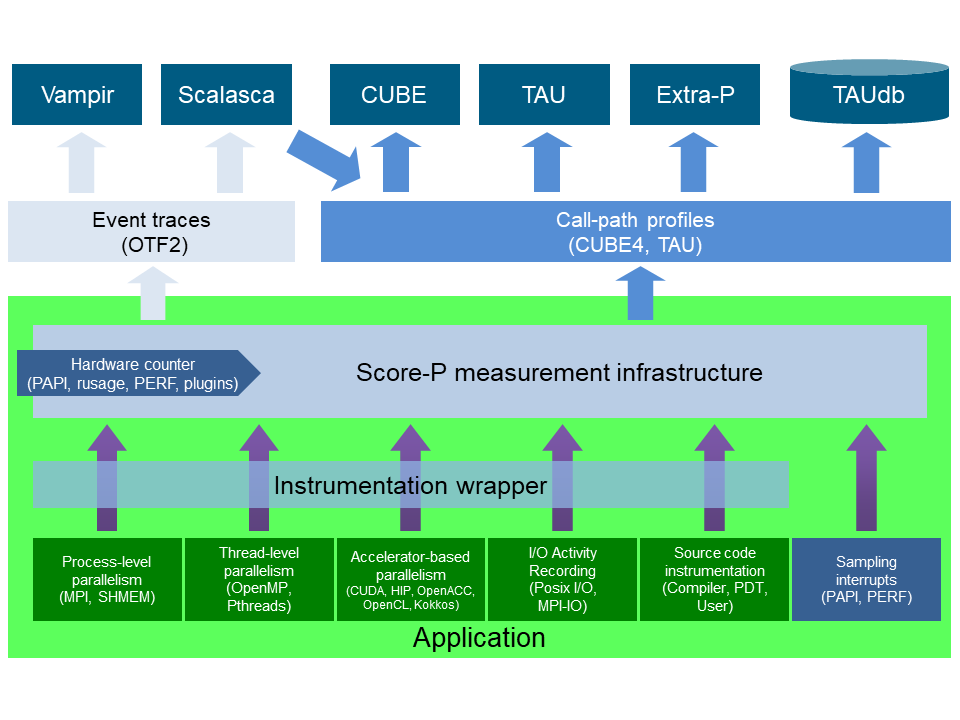
\includegraphics[width=0.75\textwidth]{score-p-overview.png}}
                {\tiny \url{https://perftools.pages.jsc.fz-juelich.de/cicd/scorep/tags/latest/html/score-p-overview.png}}
            \caption{Score-P Komponenten}
            \label{fig:score-p-overview}
        \end{center}
    \end{figure}

    Der Kern von Score-P besteht aus einer gemeinsamen Messinfrastruktur und darauf aufbauenden
    Integrationen mit unterschiedlichen Profilingschnittstellen.

    Die gesammelten Daten werden wiederum in offenen Datenformaten gespeichert und können
    dadurch von mehreren Werkzeugen verwendet werden.

    \subsubsection{Profilingschnittstellen}
    Neben manueller Instrumentierung durch den Benutzer~\longcite{Score-P-Documentation}{Application Instrumentation}
    besitzt Score-P Integrationen mit folgenden Technologien:

    \paragraph{Compilerinstrumentierung}
    Um Aufrufe von Funktionen aufzuzeichnen kann Score-P den verwendeten Compiler
    anweisen das Betreten und Verlassen dieser durch Aufrufe spezieller Funktionen
    zu markieren~\longcite{Score-P-Documentation}{Application Instrumentation}.

    Dabei ist zu beachten das die Namen der entstehenden Regionen und Art wie diese generiert
    werden von dem verwendeten Compiler abhängig ist.

    Dies ist besonders wichtig wenn die zu instrumentierende Anwendung in C++ geschrieben ist,
    weil einige Compiler kein Filtern der zu instrumentierenden Funktionen erlauben und C++
    Anwendungen häufig viele kleine Funktionen besitzen wessen Instrumentierung einen signifikanten
    Overhead erzeugen kann~\longcite{Score-P-Documentation}{Application Instrumentation}.

    \paragraph{MPI Bibliotheksaufrufe}
    Bei MPI handelt es sich um eine standardisierte Schnittstelle für den Nachrichtenaustausch
    zwischen parallel ablaufenden Prozessen mit eigenen Adressbereichen~\longcite{mpi}{1}.

    Um Aufrufe von MPI Funktionen zu Erkennen und zu Messen wird dafür das im MPI Standard
    spezifizierte `Profiling Interface'~\shortcite{mpi}{717} verwendet.

    Bei der Instrumentierung einer Anwendung wird dafür neben der MPI Implementierung zusätzlich
    gegen eine von Score-P bereitgestellte Bibliothek gelinkt~\longcite{Score-P-Documentation}{Application Instrumentation}.

    \paragraph{SHMEM Bibliotheksaufrufe}
    Bei SHMEM handelt es sich ebenfalls um eine standardisierte Schnittstelle, bei welcher jedoch
    im Gegensatz zu MPI im Rahmen des `Partitioned Global Address Space' Paradigmas von einem
    einzigen globalen Adressbereich ausgegangen wird welcher auf mehrere Ausführungseinheiten
    verteilt sein kann und Datentransfers einseitig ablaufen~\longcite{openshmem}{1}.

    Um Aufrufe von SHMEM Funktionen zu Erkennen und zu Messen wird wie bei MPI auf ein standardisiertes
    `Profiling Interface'~\shortcite{openshmem}{140} zugegriffen welches ein Linken gegen eine von
    Score-P bereitgestellte Bibliothek erfordert~\longcite{Score-P-Documentation}{Application Instrumentation}.

    \paragraph{OpenMP Direktiven und API Aufrufe}
    OpenMP ist im Gegensatz zu den beiden vorherigen Technologien keine Bibliotheksschnittstelle
    sondern eine API welche neben Funktionen auch aus Compilerdirektiven besteht.

    Damit können Anwendungsentwickler Bereiche des Quellcode explizit zur parallelen Ausführung
    innerhalb eines gemeinsamen Adressbereichs~\longcite{openmp}{23} markieren und die Umsetzung 
    dem verwendeten Compiler überlassen.

    Die Verwendung von Compilerdirektiven stellt jedoch auch eine Hürde bei der Instrumentierung dar
    weil das Erkennen und Messen von Funktionsaufrufen nicht ausreicht um die komplette API abzudecken.

    Eine der von Score-P verwendeten Lösungen stellt die Opari2 Komponente dar, welche den Quellcode der
    zu instrumentierenden Anwendung analysiert und Aufrufe von Messfunktionen an bestimmten Stellen
    einfügt~\longcite{Score-P-Documentation}{Introduction}.

    Eine Alternative ist die Verwendung des `OMPT Interface'~\shortcite{openmp}{419}, welches eine
    standardisierte Schnittstelle für die Interaktion mit einer OpenMP Implementierung darstellt.

    Zwar kann dabei auf das Modifizieren von Quellcode und die dadurch entstehende Probleme verzichtet werden,
    jedoch existiert die Schnittstelle erst seit OpenMP 5.0 und wird momentan (Stand 2024) noch nicht von
    GCC, einer weit verbreiteten Compilersammlung, unterstützt~\cite{gomp}. 

    \paragraph{Pthread Bibliotheksaufrufe}
    Pthread, auch bekannt als POSIX Threads, ist die standardisierte Threadingbibliothek auf POSIX-
    kompatiblen Betriebssystemen, welche von Score-P durch das Wrappen von Bibliothekssymbolen
    beim Linken der zu instrumentieren Anwendung mit von Score-P bereitgestellten
    Implementierungen Instrumentiert wird~\longcite{Score-P-Documentation}{Application Instrumentation}.

    \paragraph{OpenCL Bibliotheksaufrufe}
    Bei OpenCL handelt es sich wie bei MPI und SCHMEM um eine standardisierte Bibliotheksschnittstelle,
    welche es Anwendungsentwicklern erlaubt Berechnungen auf verschiedene Hardware wie u.a. einer GPU
    zu verteilen~\longcite{opencl}{2}.
    
    Dabei wird grundsätzlich von mehreren Adressbereichen ausgegangen~\longcite{openmp}{30}.

    Das Instrumentieren wird wie bei Pthread durch das Wrappen von Bibliothekssymbolen beim
    Linken ermöglicht.

    \paragraph{OpenACC Direktiven und API Aufrufe}
    Die API von OpenACC ähnelt der von OpenMP, weil der Anwendungsentwickler ebenfalls durch
    Compilerdirektiven explizit Teile der Anwendung parallel ablaufen lassen kann.

    Im Gegensatz zu OpenMP konzentriert sich OpenACC jedoch auf heterogene Hardware und besitzt
    dementsprechend meistens keinen gemeinsamen Adressbereich, da die ausgeführten Programmteile
    möglicherweise auf anderen Geräten laufen~\longcite{openacc}{11}.

    Beim Instrumentieren von Anwendungen welche OpenACC unterstützen verwendet Score-P das
    `Profiling and Error Callback Interface'~\shortcite{openacc}{123}, wofür wiederum gegen eine
    von Score-P bereitgestellte Bibliothek gelinkt~\longcite{Score-P-Documentation}{Introduction}
    werden muss.

    \paragraph{CUDA}
    CUDA ist eine vom Hersteller NVIDIA entwickelte Werkzeugsammlung welche es erlaubt GPU-basierte
    Anwendungen zu entwickeln und auszuführen~\longcite{nvidia-docs}{CUDA}.

    Score-P erlaubt das Aufzeichnen von Funktionsaufrufen der CUDA API und GPU Aktivitäten mit Hilfe des
    `CUDA Profiling Tools Interface'~\shortcite{nvidia-docs}{CUPTI}~\longcite{Score-P-Documentation}{Application Measurement}.

    \paragraph{HIP}
    Bei HIP handelt es sich wie bei CUDA um eine Werkzeugsammlung für die Entwicklung von GPU-basierten
    Anwendungen welche vom Hersteller AMD als Bestandteil der ROCm Plattform mit einem Fokus auf
    Kompatibilität mit GPUs von sich selbst und NVIDIA entwickelt wurde~\longcite{rocm-docs}{HIP documentation}.

    Wie bei CUDA unterstützt Score-P das Aufzeichnen von Funktionsaufrufen der ROCm API und GPU Aktivitäten,
    wobei eine nicht näher spezifizierte Schnittstelle verwendet wird~\longcite{Score-P-Documentation}{Application Measurement}.

    \paragraph{I/O}
    Funktionsaufrufe von Funktionen bekannter I/O Schnittstellen können durch Score-P aufgezeichnet werden.

    Dabei werden neben den bekannten POSIX Funktionen auch Funktionen der asynchronen POSIX Schnittstelle,
    ISO C und MPI unterstützt~\longcite{Score-P-Documentation}{Introduction}.

    \subsubsection{Datenformate}
    Nach dem Instrumentieren einer Anwendung ermöglicht Score-P zwei Arten der Datenerfassung,
    genannt `tracing' und `profiling'.

    Bei `tracing' werden aufzuzeichnende Ereignisse unter Beibehaltung zeitlicher und örtlicher
    Zusammenhänge im Open Trace Format 2 abgespeichert, welches u.a. von den Werkzeugen Scalasca
    und Vampir verwendet wird~\longcite{Score-P-Documentation}{Application Measurement}.

    Da dies jedoch gro{\ss}e Datenmengen erzeugen kann erlaubt `profiling' das Zusammenfassen von
    Ereignissen innerhalb bestimmter Regionen, wobei die entstehenden Daten im CUBE4 Format
    gespeichert und von Werkzeugen wie Cube und TAU verwendet werden
    können~\longcite{Score-P-Documentation}{Application Measurement}.

    Dabei stellt jede aufgerufene Funktion eine Region dar welche zusammen mit den von ihr
    aufgerufenen Funktionen einen Baum bildet.

    Die entstehenden Aufrufbäume können basierend auf bestimmten Funktionsparametern,
    benutzerdefinierten Phasen und einzelnen Aufrufen weiter unterteilt
    werden~\longcite{Score-P-Documentation}{Application Measurement}.

    \subsection{Anwendung}
    Um eine Anwendung mit Score-P zu instrumentieren wird ein Befehl namens \texttt{scorep} zur Verfügung
    gestellt welcher vor die Befehle zum Kompilieren und Linken der Anwendung gestellt wird.

    Das damit assoziierte Programm analysiert den übergebenen Befehl und führt die zur Instrumentierung
    notwendigen Aktionen aus, wobei die Berechnung von benötigten Linkerargumenten und zu linkenden
    Bibliotheken von einem weiteren Werkzeug namens \texttt{scorep-config} durchgeführt
    wird~\longcite{Score-P-Documentation}{Score-P Tools}.

    Die zu nutzenden Profilingschnittstellen werden über Befehlsargumente ausgewählt oder durch
    Analyse des übergebenen Befehls erkannt, wobei letzteres nicht immer funktioniert~\longcite{Score-P-Documentation}
    {Application Instrumentation}.

    Dabei ist zu beachten dass für jede instrumentierte Anwendung nur ein Threading Paradigma
    (OpenMP oder Pthread) und eine Kommunikationsparadigma (MPI oder SHMEM) ausgewählt werden kann
    und es Einschränkungen bei der Verwendung von Profilingschnittstellen in statischen
    Bibliotheken gibt wenn diese nicht beim Erstellen der fertigen Anwendung aktiviert werden.

    Zusätzlich kann die Unterstützung für bestimmte Profilingschnittstellen bei einer Score-P
    Installation fehlen, was durch die Ausgaben des Befehls \texttt{scorep-info} überprüft werden kann.

    Au{\ss}erdem kann bei der Verwendung von Werkzeugen wie CMake und Autotools der konfigurierte Compiler
    bereits vor dem Bauen eines Projektes aufgerufen werden um die Verfügbarkeit von Schnittstellen
    oder andere Informationen für das Konfigurieren des Projektes zu erhalten.

    Da bei der Verwendung von Score-P der \texttt{scorep} Befehl als Compiler verwendet wird kann es dabei
    zu Fehlern kommen obwohl Score-P in dieser Phase nicht benötigt wird~\longcite{Score-P-Documentation}
    {Score-P Compiler Wrapper Usage}.

    Um dies zu verhindern stellt Score-P Befehle bereit welche sich normalerweise wie der Befehl
    \texttt{scorep} verhalten, durch das Setzen von bestimmten Umgebungsvariablen jedoch den Aufruf an den
    verwendeten Compiler durchreichen~\longcite{Score-P-Documentation}{Score-P Compiler Wrapper Usage}.

    \newpage
    \section{Betrachtung CMake}
    Bei CMake handelt es sich um ein Werkzeug zum Bauen von Softwareprojekten, welches aus in einer
    plattformunabhängigen Sprache definierten Projektbeschreibung die dafür nötigen Schritte
    ermittelt~\longcite{CMake-Documentation}{User Interaction Guide}.

    Die Verwendung von CMake besteht zuerst auf einer Konfigurationsphase in welcher Informationen
    über das aktuelle System gesammelt und die Projektbeschreibung evaluiert wird.
    Zusätzlich können Optionen deklariert werden welche es ermöglichen Einfluss auf den
    Konfigurationsprozess zu nehmen.
    Anschlie{\ss}end wird mit den gesammelten Daten eine Konfiguration für ein plattformspezifisches Werkzeug
    (wie u.a. Unix Makefiles oder Visual Studio~\longcite{CMake-Documentation}{cmake-generators(7)})
    generiert welches das eigentliche Bauen des Projektes
    übernimmt~\longcite{CMake-Documentation}{User Interaction Guide}.

    \subsection{Projektbeschreibung}
    Die Projektbeschreibung ist in einer CMake spezifischen Sprache verfasst welche die Zeichenkette
    als einzigen Datentyp besitzt, wobei Zeichenketten als Werte anderer Datentypen interpretiert
    werden können~\longcite{CMake-Documentation}{cmake-language(7)}.
    Sie besteht aus mehreren `Targets' welche Befehle zum Erreichen eines bestimmten Zustandes wie
    z.B. das Bauen eines ausführbaren Programms repräsentieren~\longcite{CMake-Documentation}{cmake-buildsystem(7)}.
    Ein Target kann von den Ergebnissen anderer Targets abhängen, was dafür sorgt dass vor der
    Ausführung der Befehle eines abhängigen Targets die Befehle der referenzierten Targets ausgeführt werden.

    \subsubsection{Targettypen}
    Neben benutzerdefinierten Targets besitzt CMake bereits vordefinierte Targets zum repräsentieren
    von häufigen Aktionen beim Bauen von Programmen, welche nachfolgend erläutert
    werden~\longcite{CMake-Documentation}{cmake-buildsystem(7)}.

    \paragraph{\texttt{EXECUTABLE}} Targets repräsentieren ausführbaren Programme.

    \paragraph{\texttt{STATIC\_LIBRARY}} Targets repräsentieren statische Programmbibliotheken welche
    beim Linken anderer Programmteile verwendet werden können.

    \paragraph{\texttt{SHARED\_LIBRARY}} Targets repräsentieren dynamische Programmbibliotheken welche
    neben dem Linken anderer Programmteile auch zur Laufzeit geladen werde kann.

    \paragraph{\texttt{MODULE\_LIBRARY}} Targets repräsentieren dynamische Programmkomponenten welche
    im Gegensatz zu Bibliotheken nur zur Laufzeit geladen werden.

    \paragraph{\texttt{OBJECT\_LIBRARY}} Targets repräsentieren Mengen von bereits zu Objektcode
    kompilierten Quelltexten.

    \paragraph{\texttt{INTERFACE\_LIBRARY}} Targets repräsentieren Ausführungskonfigurationen welche andere
    Targets durch linken übernehmen können.

    \paragraph{\texttt{ALIAS}} Targets repräsentieren andere Targets und können im Gegensatz zu vielen
    anderen Targets nicht verändert werden.

    \paragraph{\texttt{IMPORTED}} Targets repräsentieren bereits existierende Objekte welche z.B. durch
    installierte Programme zur Verfügung gestellt werden und können deswegen nicht bearbeitet
    oder erneut gebaut werden.

    \subsubsection{Targeteigenschaften}
    CMake definiert bestimmte Targeteigenschaften welche die Ausführung eines Target beeinflussen,
    wobei eine Auswahl nachfolgend erläutert wird~\longcite{CMake-Documentation}{cmake-properties(7)}.

    An vielen Stellen erlaubt CMake die Verwendung sogenannter `generator expressions', was spezielle
    Ausdrücke sind welche nach der Evaluation der Projektbeschreibung beim Generieren der Werkzeugkonfiguration
    ausgewertet werden~\longcite{CMake-Documentation}{cmake-generator-expressions(7)}.
    Sie erlauben bei Werkzeugen welche mehrere Konfigurationsprofile besitzen ein Anpassen von
    Eigenschaftswerten an das benutzte Profil, was bei der Evaluation der Projektbeschreibung
    noch unbekannt ist und erst im Rahmen der Konfigurationsgenerierung ermittelt werden kann.

    \paragraph{\texttt{<LANG>\_COMPILER\_LAUNCHER}} enthält ein Programm welches verwendet werden soll um
    Aufrufe des Compiler einer bestimmten Programmiersprache durchzuführen.
    Die Unterscheidung nach der zu kompilierenden Programmiersprache wird benötigt weil CMake es erlaubt
    dass Targets welche Quellcodedateien verarbeiten (wie zum Beispiel solche vom Typ \texttt{EXECUTABLE})
    Quellcodedateien von unterschiedlichen Programmiersprachen zugewiesen bekommen.
    In diesem Fall werden die einzelnen Quellcodedateien mit dem ihrer Programmiersprache zugewiesenen
    Compiler kompiliert und anschlie{\ss}end durch den Linker einer der Sprachen zu dem gewünschten Ergebnis
    (wie zum Beispiel einer ausführbaren Datei) gelinkt.

    \paragraph{\texttt{<LANG>\_LINKER\_LAUNCHER}} verhält sich wie \texttt{<LANG>\_COMPILER\_LAUNCHER}
    für Aufrufe des Linkers, ist jedoch nur für die Programmiersprachen C, C++ und Objective-C implementiert.
    In praktischen Versuchen wurde ermittelt dass auch für andere Programmiersprachen Linker in CMake
    existieren, diese jedoch diese Eigenschaft ignorieren.
    Um Programmiersprachen wie CUDA trotzdem durch einen Linker Launcher linken zu lassen kann durch die
    Eigenschaft \texttt{LINKER\_LANGUAGE} der Linker einer unterstützten Sprache wie C++ verwendet werden.

    \paragraph{\texttt{LINK\_LIBRARIES}} enthält Bibliotheken oder Targets gegen welche das Target gelinkt
    werden soll wobei die Verwendung von `generator expressions' erlaubt ist.

    \paragraph{\texttt{INTERFACE\_LINK\_LIBRARIES}} enthält Bibliotheken oder Targets gegen welche beim Linken
    gegen das aktuelle Target zusätzlich gelinkt werden soll wobei die Verwendung von
    `generator expressions' erlaubt ist.

    Dabei ist es unerheblich ob das Linken im Rahmen von \texttt{LINK\_LIBRARIES} oder durch Verweise
    in \texttt{INTERFACE\_LINK\_LIBRARIES} anderer gelinkter Targets stattfindet.

    \subsection{Module}
    CMake erlaubt es Benutzern Programme welche in der CMake Sprache geschrieben sind wiederzuverwenden
    indem deren Quellcode innerhalb des aktuellen Namensraumes für Variablen durch die \texttt{include}
    Funktion evaluiert wird~\longcite{CMake-Documentation}{include}.
    Dabei kann eine bestimmte Datei oder nur der Name des zu ladenden Moduls angegeben werden,
    in welchem Falle die den Quellcode des Moduls enthaltene Datei in Verzeichnissen welche in
    der Variable \texttt{CMAKE\_MODULE\_PATH} gespeichert sind gesucht wird.

    Dem gegenüber steht der Begriff des `Package', welcher externe Software welche durch den
    Benutzer beim Bauen des Projektes angefordert werden kann
    beschreibt~\longcite{CMake-Documentation}{cmake-packages(7)}.
    Diese Software wird au{\ss}erhalb von CMake durch den Benutzer installiert und besteht aus
    Sicht von CMake aus importierten Targets oder Variablen mit weiteren Informationen, wobei
    zwei Arten von Packages mit unterschiedlichen Lokalisierungsmechanismen existieren.

    Die erste Art nutzt Module welche den Namen der zu lokalisierenden Software mit einem `Find'
    Präfix tragen und beim Aufruf die zur Lokalisierung der Software notwendigen Schritte
    durchführen~\longcite{CMake-Documentation}{cmake-developer(7)}.
    Dabei müssen diese Module nicht von der zu lokalisierenden Software bereitgestellt werden sondern
    können auch durch den Benutzer in von CMake durchsuchten Verzeichnissen abgelegt werden.

    Die zweite Art nutzt eine Reihe von CMake Dateien mit dem Namen der Software und den Postfix `Config'
    und `Version' welche im Gegensatz zu Find-Modulen zu einer bestimmten Installation der Software
    gehören und von der zu lokalisierenden Software bereitgestellt
    werden~\longcite{CMake-Documentation}{cmake-packages(7)}.
    Dadurch kann ein möglicherweise aufwendiges Untersuchen der Installation auf bestimmte Merkmale
    vermieden werden, jedoch setzt dies voraus dass die zu lokalisierende Software mit CMake
    gebaut wurde oder diese Dateien manuell generiert werden.

    Unabhängig von der Art des Package kann bei dessen Suche eine Versionsnummer
    (im Format Major.Minor.Patch.Tweak) und eine Liste von Komponenten übergeben
    werden~\longcite{CMake-Documentation}{find\_package}.
    Da es sich wie bei allen Variablen in CMake bei ihnen um Zeichenketten handelt ist die Verarbeitung
    der Versionsnummer und Definition der Komponenten abhängig von der Implementierung des Package,
    jedoch ist vorgesehen dass die Version der lokalisierten Software kompatibel zu der übergebenen
    Versionsnummer ist und die lokalisierte Installation die als benötigt deklarierte Komponenten
    besitzt~\longcite{CMake-Documentation}{find\_package}.

    \newpage
    \section{Implementierung}
    Die Implementierung besteht aus zwei getrennten Modulen um die unabhängige Verwendung dieser
    zu ermöglichen.

    \subsection{Lokalisierungsmodul}
    Zum Lokalisieren einer Score-P Installation wurde das Modul `FindScoreP' entwickelt weil
    durch die fehlende Verwendung von CMake durch Score-P die Verwendung von Config-Modulen
    ein manuelles Generieren der benötigten CMake Dateien vorausgesetzt hätte.
    Es unterstützt neben Versionsnummern, welche mit der Funktion \texttt{find\_package\_check\_version}
    auf Kompatibilität hin überprüft werden, das Finden einer kompatiblen Version wenn
    mehrere verschiedene Versionen von Score-P installiert sind.

    \subsubsection{Komponenten}
    Da eine Score-P Installation Einschränkungen in den unterstützten Profilingschnittstellen und
    andere Eigenschaften welche für die zu instrumentierende Anwendung von Bedeutung sind besitzen
    kann können diese durch Komponenten abgefragt werden.
    Das Vorhandensein einer Komponente wird durch die Analyse der Ausgabe des Befehls
    \texttt{scorep-info config-summary} ermittelt, wobei die verfügbaren Komponenten und ihre
    Bedeutungen nachfolgend erläutert werden.

    \paragraph{\texttt{<BACKEND>COMPILER\_<SPRACHE>\_<COMPILER>}} repräsentiert den von einem Score-P Backend
    zum Kompilieren einer Sprache verwendeten Compiler, wobei die Backends \texttt{MPI\_} für MPI,
    \texttt{SHMEM\_} für SHMEM und das leere Backend für den standardmä{\ss}ig verwendeten Compiler existieren.
    Dies ermöglicht es sicherzustellen dass der von Score-P verwendete Compiler mit dem Compiler
    welcher für das zu instrumentierende Projekt konfiguriert wurde übereinstimmt.

    \paragraph{\texttt{MPP\_<PARADIGMA>}} repräsentiert die Unterstützung für ein bestimmtes Paradigma zur
    Verwendung mehrerer Prozesse, wobei die Paradigmas \texttt{mpi} für MPI und \texttt{shmem} für SHMEM existieren.

    \paragraph{\texttt{IO\_<PARADIGMA>}} repräsentiert die Unterstützung für ein bestimmtes Paradigma zur
    Aufzeichnung von I/O Operationen, wobei nur das Paradigma \texttt{posix} für POSIX Schnittstellen existiert.

    \paragraph{\texttt{COMPILER}} repräsentiert die Unterstützung für Compilerinstrumentierung.

    \paragraph{\texttt{CUDA}} repräsentiert die Unterstützung für CUDA.
    
    \paragraph{\texttt{POMP}} repräsentiert die Unterstützung für eine nicht näher beschriebene Schnittstelle
    names `OPARI2 pomp user instrumentation'.

    \paragraph{\texttt{OMP\_<SPRACHE>}} repräsentiert die Unterstützung von OpenMP für eine bestimmte Sprache.

    \paragraph{\texttt{OPARI2}} repräsentiert die Verfügbarkeit von Opari2.

    \paragraph{\texttt{OMPT}} repräsentiert die Unterstützung der OMPT Schnittstelle.

    \paragraph{\texttt{PDT}} repräsentiert die Unterstützung einer nicht näher beschriebenen Schnittstelle
    namens `PDT'.

    \paragraph{\texttt{OPENCL}} repräsentiert die Unterstützung von OpenCL.

    \paragraph{\texttt{OPENACC}} repräsentiert die Unterstützung von OpenACC.

    \paragraph{\texttt{MEMORY}} repräsentiert die Unterstützung des Aufzeichnens der Speicherverwendung.

    \paragraph{\texttt{LIBWRAP}} repräsentiert die Unterstützung von Bibliothekswrappern.

    \paragraph{\texttt{KOKKOS}} repräsentiert die Unterstützung von Kokkos.

    \paragraph{\texttt{HIP}} repräsentiert die Unterstützung von HIP.

    \subsubsection{Lokalisierungsmechanismus}
    Der Mechanismus zum Lokalisieren einer Score-P Installation wird nachfolgend erläutert.

    \begin{enumerate}
        \item Lokalisieren von \texttt{scorep-config}

        Dies wird für das Ermitteln des Installationsortes benötigt und durch die CMake Funktion \\
        \texttt{find\_program} durchgeführt.
        Dabei wird bereits für jede lokalisierte Installation überprüft ob diese mit der übergebenen
        Version und den übergebenen Komponenten kompatibel ist um im Falle von mehreren Installationen
        jene zu ignorieren welche nicht kompatibel sind.

        \item Ermitteln der Version und des Installationsortes

        Dies wird durch die Befehle \texttt{scorep-config --version} und \texttt{scorep-config --prefix} erreicht.

        \item Lokalisieren von \texttt{scorep} und \texttt{scorep-info}

        Dabei kommt wieder die Funktion \texttt{find\_program} zum Einsatz wobei die Suche auf den Installationsort
        beschränkt wird um zu verhindern dass Programme anderer Installationen lokalisiert werden.

        \item Überprüfen des Vorhandenseins übergebener Komponenten

        Obwohl dies beim Lokalisieren von \texttt{scorep-config} bereits durchgeführt wurde wird es erneut
        durchgeführt um bei der Ermittlung des Lokalisierungsergebnisses benötigte Variablen zu setzen.

        \item Erstellen importierter Targets

        Dieser Schritt wird übersprungen falls die Lokalisierung im Rahmen eines CMake Scripts
        durchgeführt wird und deswegen keine Targets erstellt werden können.

        \item Ermitteln des Lokalisierungsergebnisses

        Dies sorgt dafür das unter anderem Variablen gesetzt werden welche CMake signalisieren ob das
        Lokalisieren erfolgreich war.
        Weil die dafür von CMake bereitgestellte Funktion \\ \texttt{find\_package\_handle\_standard\_args}
        Informationen über die existierenden Komponenten in Form von gesetzten Variablen benötigt wird deren
        Vorhandensein vorher erneut überprüft.
    \end{enumerate}
    
    \subsubsection{Ausgaben}
    Im Falle der erfolgreichen Lokalisierung einer Score-P Installation werden die folgenden
    Targets und Variablen erstellt.

    \paragraph{\texttt{ScoreP::ScoreP}} ist ein importiertes Target welches die ausführbare Datei
    des \texttt{scorep} Befehls repräsentiert.
    Der Pfad dieser Datei wird zusätzlich in der Variable \texttt{SCOREP\_EXECUTABLE} gespeichert.

    \paragraph{\texttt{ScoreP::Config}} ist ein importiertes Target welches die ausführbare Datei
    des \texttt{scorep-config} Befehls repräsentiert.
    Der Pfad dieser Datei wird zusätzlich in der Variable \\ \texttt{SCOREP\_CONFIG\_EXECUTABLE} gespeichert.

    \paragraph{\texttt{ScoreP::Info}} ist ein importiertes Target welches die ausführbare Datei
    des \texttt{scorep-info} Befehls repräsentiert.
    Der Pfad dieser Datei wird zusätzlich in der Variable \texttt{SCOREP\_INFO\_EXECUTABLE} gespeichert.

    \paragraph{\texttt{SCOREP\_FOUND}} ist eine Variable welche einen Wahrheitswert enthält der angibt
    ob die Lokalisierung erfolgreich war.

    \paragraph{\texttt{SCOREP\_<KOMPONENTE>\_FOUND}} ist eine Variable welche einen Wahrheitswert enthält
    der angibt ob eine bestimmte übergebene Komponente gefunden wurde.

    \paragraph{\texttt{SCOREP\_VERSION\_STRING}} ist eine Variable welche die Version der lokalisierten
    Score-P Installation enthält.

    \subsection{Instrumentierungsmodul}
    Um ein von CMake verwaltetes Projekt zu Instrumentieren stellt dass Modul `ScorePUtilites'
    Funktionen bereit welche sich in eine Low- und High-Level Schnittstelle unterteilen.

    \subsubsection{Low-Level Schnittstelle}
    Die Low-Level Schnittstelle ist darauf ausgerichtet den Entwickler einer Anwendung bei deren
    Instrumentierung zu unterstützen und Ihm dabei grö{\ss}tmögliche Kontrolle zu ermöglichen.

    Dafür wird eine Funktion namens \texttt{scorep\_instrument} bereitgestellt welche es erlaubt eine Liste
    von übergebenen Targets für die Verwendung von Score-P zu konfigurieren.
    Dies wird erreicht indem für alle zu instrumentierenden Programmiersprachen die Targeteigenschaften
    \texttt{<LANG>\_COMPILER\_LAUNCHER} und \texttt{<LANG>\_LINKER\_LAUNCHER} auf den zu verwendenden
    Score-P Befehl gesetzt werden um das Kompilieren und Linken von Score-P durchführen zu lassen.

    Dabei muss durch den Entwickler eine Liste der vom Target verwendeten Programmiersprachen übergeben
    werden weil eine Analyse des Targets durch die Möglichkeit der Verwendung von Generatorausdrücken 
    beim Konfigurieren des CMake Projekts nicht vollständig möglich ist.
    Wenn der Benutzer jedoch die Unvollständigkeit der Analyse für unproblematisch befindet
    kann diese optional verwendet werden um aus den Abhängigkeiten eines Targets seine Score-P
    Einstellungen abzuleiten.

    Au{\ss}erdem muss eine mit den gewählten Befehlen kompatible Score-P Installation vor der Verwendung
    der Schnittstelle durch das Lokalisierungsmodul lokalisiert werden um den Speicherort des
    Score-P Befehls zu ermitteln.

    Der Vorteil von Targeteigenschaften im Vergleich zur Verwendung von einem von Score-P bereitgestellten
    Compilerwrappers ist neben der Fähigkeit der selektiven Instrumentierung von Teilen eines Projektes
    die automatische Verwendung des vom Nutzer konfigurierten Compilers beim Konfigurieren des Projektes.

    \subsubsection{High-Level Schnittstelle}
    Da wie bereits erwähnt Einschränkungen bei der Auswahl verschiedener Score-P Einstellungen wie zum
    Beispiel des zu verwendenden Threading Paradigmas existieren kann es bei der manuellen Instrumentierung
    von einzelnen Targets zu fehlerhaften Konfigurationen kommen.
    Um dies zu vermeiden existiert neben der Low-Level Schnittstelle eine High-Level Schnittstelle
    welche es dem Entwickler der zu instrumentieren Anwendung erlaubt im Austausch für Kontrolle
    über den Instrumentierungsprozess erforderliche Score-P Einstellungen automatisch zu ermitteln.
    Diese Schnittstelle sieht vor dass im Gegensatz zur Low-Level Schnittstelle die Instrumentierung
    in mehreren Phasen erfolgt um die übergebenen Informationen zu analysieren.

    Zuerst werden die zu instrumentierenden Targets mit der Funktion \texttt{scorep\_mark} über Targeteigenschaften
    als solche markiert und die gewünschten Score-P Einstellungen mit einer vom Benutzer vorgegebenen
    Priorität gespeichert.
    Die Priorität ermöglicht es bei der Targetanalyse dem Benutzer seine Präferenzen im Falle von
    in Konflikt stehenden Einstellungswerten auszudrücken.

    Anschlie{\ss}end wird mit der Funktion \texttt{scorep\_determine\_instrumentations} durch eine Analyse der Targets
    die endgültigen Score-P Einstellungen ermittelt und ebenfalls als Targeteigenschaften gespeichert.

    Zum Schluss wird eine Score-P Installation lokalisiert und mit der Funktion \texttt{scorep\_enable}
    die ermittelten Einstellungen über die Low-Level Schnittstelle angewendet, wobei die im vorherigen
    Schritt erfolgte Analyse die zur Instrumentierung benötigten Komponenten ermitteln kann.

    \subsubsection{Targetanalyse}
    Die zum Ermitteln der endgültigen Score-P Einstellungen durchgeführte Targetanalyse der High-Level
    Schnittstelle wird an der in Abbildung~\ref{fig:analysis_before} dargestellten Beispielkonfiguration
    von Targets erläutert, wobei rote Targets zum Instrumentieren markiert wurden.
    Dabei ist zu beachten dass es sich bei den analysierten Abhängigkeiten nur um solche handelt
    welche keine Generatorausdrücke verwenden weil diese sonst nicht während des Konfigurierens
    des CMake Projekts evaluiert werden können.

    \begin{figure}
        \begin{center}
            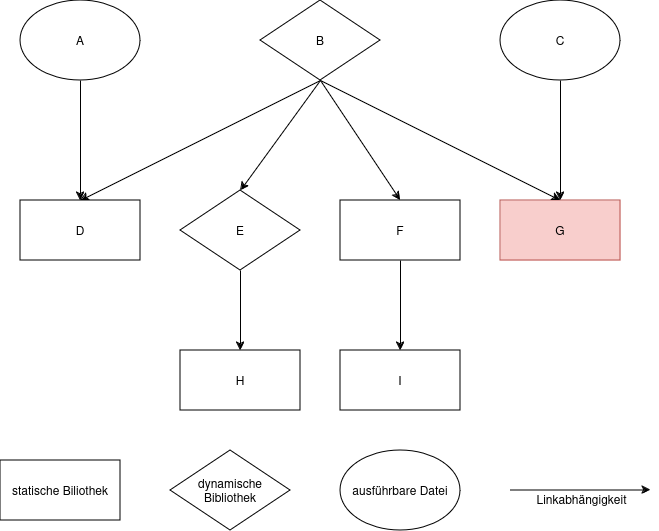
\includegraphics[width=0.75\textwidth]{analysis_before.drawio.png}
            \caption{Beispiel einer Projektkonfiguration vor der Targetanalyse}
            \label{fig:analysis_before}
        \end{center}
    \end{figure}

    In dem Beispiel existieren eine Reihe von Targets mit durch Pfeile dargestellten Abhängigkeiten
    beim Linken, welche neben statischen Bibliotheken sogenannte `standalone Targets' beinhalten.
    Diese `standalone Targets' beinhalten alle Targettypen von CMake welche einen sogenannten
    Konstruktor besitzen und damit im Rahmen der meisten Score-P Einstellungen nicht an die
    sie benutzenden Anwendung gebunden sind, wozu neben \texttt{EXECUTABLE} und \texttt{SHARED\_LIBRARY}
    auch Targets des Typs \texttt{MODULE\_LIBRARY} zählen.
    Im Gegensatz dazu besitzen statische Bibliotheken keinen eigenen Konstruktor und müssen deswegen
    die gleichen Score-P Einstellungen wie die Programme verwenden in welche sie gelinkt werden, was
    dazu führen kann dass Targets welche ursprünglich nicht als zu instrumentierend markiert wurden
    trotzdem instrumentiert werden müssen wenn sie gegen eine als solche markierte statische
    Bibliothek linken.

    Um diese Einschränkungen nicht zu verletzen werden Mengen von Targets ermittelt welche im
    Hinblick auf eine Menge von Score-P Einstellungen im Falle einer Instrumentierung durch
    Score-P die gleichen Einstellungswerte besitzen müssen.

    Die erste Art dieser Mengen wird im nachfolgendem Text `lokale Abhängigkeiten' genannt und
    besteht für jedes standalone Target aus seinen transitiven Abhängigkeiten welche sich
    seinen Konstruktor teilen.
    Innerhalb dieser Mengen darf nur eine Score-P Konfiguration existieren welche auf alle zu
    instrumentierenden Targets angewendet wird, wobei im Falle von instrumentierten Abhängigkeiten
    das der Menge zugeordnete standalone Target ebenfalls instrumentiert wird falls dies nicht
    bereits dazu markiert wurde.

    Um eindeutige Threading und Kommunikationsparadigma auch über Abhängigkeiten mit eigenen
    Konstruktoren hinweg sicherzustellen existiert zusätzlich eine zweite Art von Mengen, welche
    nachfolgend `globale Abhängigkeiten' genannt werden.
    Diese Mengen sind Erweiterungen der lokalen Abhängigkeiten welche zusätzlich alle transitiven
    Abhängigkeiten enthalten und nur die verwendeten Threading und Kommunikationsparadigma einschränken.

    Gleichzeitig kann ein Target nicht mit mehreren unterschiedlichen Score-P Konfigurationen
    instrumentiert werden, was zu Konflikten führen kann wenn ein Target in mehreren dieser
    Mengen enthalten ist und für diese unterschiedliche Score-P Einstellungen ermittelt werden.
    Um dies zu verhindern werden Mengen welche sich zu instrumentierende Targets mit anderen
    Mengen teilen mit diesen vereint, wobei eine Union-Find-Datenstruktur zum Einsatz kommt.

    \begin{figure}
        \begin{center}
            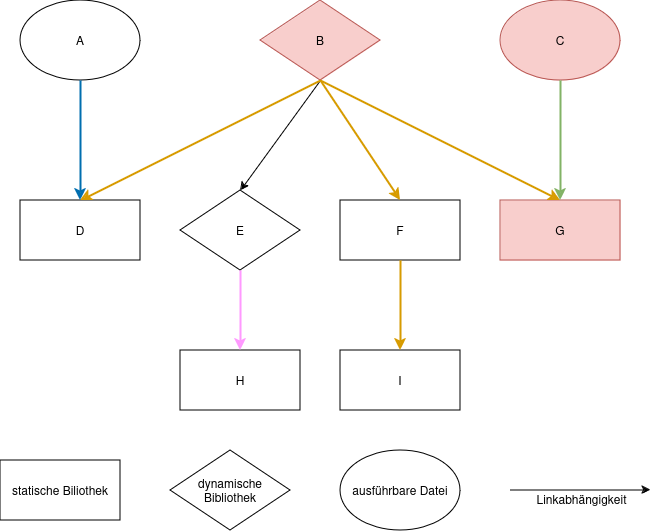
\includegraphics[width=0.75\textwidth]{analysis_localsets.drawio.png}
            \caption{Beispiel einer Projektkonfiguration nach der Targetanalyse}
            \label{fig:analysis_localsets}
        \end{center}
    \end{figure}

    Um diesen Vorgang zu veranschaulichen wurde in Abbildung~\ref{fig:analysis_localsets} die
    Targetanalyse durchgeführt und die lokalen Abhängigkeiten jedes standalone Targets vor eventuellen
    Vereinigungen mit anderen lokalen Abhängigkeiten farblich markiert.
    Es ist ersichtlich dass die dynamische Bibliothek E und alle ihre Abhängigkeiten nicht zu den
    lokalen Abhängigkeiten von B gehören weil sie durch das Linken in die dynamische Bibliothek E
    deren Konstruktor verwenden falls sie nicht bereits einen besitzen.

    Zusätzlich wurden neben dem bereits als zu instrumentierend markierten statischen Bibliothek G
    die standalone Targets B und C ebenfalls markiert weil deren lokale Abhängigkeiten dementsprechend
    markierte Targets besitzen.
    Ohne diesen Schritt könnte der Konstruktor dieser beiden Targets nicht von Score-P modifiziert und
    dementsprechend eine fehlerhafte dynamische Bibliothek oder ausführbare Datei erstellt werden.
    Jedoch kommt es nun dazu das G in den lokalen Abhängigkeiten von beiden Targets enthalten ist,
    was es ermöglicht zwei unterschiedliche Score-P Einstellungen für G zu ermitteln.
    Da G jedoch nur eine der Score-P Einstellungen verwenden kann muss dies verhindert werden.

    Aus diesem Grund würden bei der Ermittlung der Score-P Einstellungen die lokalen Abhängigkeiten
    von B und C vereinigt und ein Konflikt dadurch ausgeschlossen werden.
    Obwohl eine ähnliche Situation für die statische Bibliothek D existiert würde in diesem Fall keine
    Vereinigung der lokalen Abhängigkeiten von A und B durchgeführt weil D im Gegensatz zu G nicht
    als zu instrumentierend markiert wurde und durch die ausbleibende Anwendung ein Konflikt zwischen
    unterschiedlichen Score-P Einstellungen nicht auftreten kann.

    Schlussendlich würde dies bedeuten dass bei einem analogen Verfahren für die globalen Abhängigkeiten
    folgende Mengen existieren:
    \begin{align*}
        \text{lokale Abhängigkeiten} &= \{ \{ B, D, F, I, G, C \}, \{ A, D \}, \{ E, H \} \} \\
        \text{globale Abhängigkeiten} &= \{ \{ B, D, F, I, G, C, E, H \}, \{ A, D \}, \{ E, H \} \}
    \end{align*}

    Da einige Mengen keine zu instrumentierenden Targets enthalten können diese ignoriert werden
    weil durch den fehlenden Bedarf an Score-P Einstellungen deren Ermittlung für diese Mengen
    nutzlos wäre.

    Zusätzlich könnten aus allen Mengen nicht zu instrumentierende Targets entfernt werden weil
    diese ohne Score-P Instrumentierung keine Einstellungen besitzen und deswegen beim Ermitteln
    der Score-P Einstellungen das Ergebnis im Falle einer Abwesenheit nicht verändern würden.
    Jedoch bietet die Funktion \texttt{scorep\_mark} die Möglichkeit Targets mit Score-P Einstellungen
    zu versehen ohne sie als zu instrumentierend zu markieren.
    Dies ermöglicht es den Benutzern die Score-P Einstellungen von gegen ein bestimmtes Target linkenden
    Targets zu beeinflussen ohne dabei das gelinkte Target ebenfalls instrumentieren zu müssen.

    Falls für eine Score-P Einstellung mehrere Werte innerhalb einer Menge existieren müssen diese
    zusammengeführt oder falls dies nicht möglich ist ein Fehler gemeldet werden.
    Bei dem Zusammenführen von zwei Einstellungswerten wird zuerst versucht den Wert mit der höchsten
    Priorität zu verwenden.
    Ist dies aufgrund gleicher Prioritäten nicht möglich wird versucht ob die beiden Werte kompatibel
    sind, was zum Beispiel der Fall sein kann wenn es sich um die selben Werte handelt oder ein
    Wert eine spezifischere Version des anderen darstellt.
    Ist dies ebenfalls nicht möglich wird ein Konflikt gemeldet, wobei dies bis zum Zusammenführen
    aller Einstellungswerte verzögert wird um das Überschreiben des Konfliktes zu ermöglichen falls
    andere Werte mit einer höheren Priorität existieren.


    \newpage
    \section{Leistungsanalyse}
    Zur Beurteilung der Nützlichkeit der entwickelten CMake Module wird nachfolgend deren Anwendung
    am Beispiel der GROMACS~\cite{gromacs} Anwendung gezeigt und mit Alternativen verglichen.

    \subsection{bisherige Umsetzung}
    Die bisherige Umsetzung bestand wie in Listing~\ref{lst:wrapper} dargestellt aus der Verwendung der
    Score-P Wrapper~\longcite{Score-P-Documentation}{Score-P Compiler Wrapper Usage}, welche wie bei
    der Betrachtung von Score-P bereits erwähnt das Setzen von bestimmten Umgebungsvariablen vor dem
    Konfigurieren des CMake Projekts voraussetzt.

    \begin{lstlisting}[caption=Anwendung eines Score-P Wrapper bei GROMACS, language=bash, gobble=8, label=lst:wrapper]
        export SCOREP_WRAPPER_INSTRUMENTER_FLAGS= \
        "--thread=omp:ompt --io=posix --compiler"
        SCOREP_WRAPPER=off cmake -S . -B build -DGMX_BUILD_OWN_FFTW=ON \
        -DCMAKE_CXX_COMPILER=scorep-clang++
    \end{lstlisting}

    Neben einer Konfiguration des Projektes au{\ss}erhalb der von CMake dafür vorgesehen Mechanismen
    wie zum Beispiel der CMake Sprache erlaubt es diese Umsetzung aufgrund der Verwendung globaler
    Umgebungsvariablen nicht die Instrumentierung einzelner Targets zu steuern.
    Dies sorgt in diesem Beispiel dafür dass ein in Score-P existierender Fehler welcher durch das
    fehlerhafte Linken von statischen Bibliotheken ein Bauen der Anwendung unmöglich macht
    nur unter hohen Aufwand umgangen werden könnte.

    Zusätzlich wird der Konfigurationsprozess des Projektes komplizierter weil neben dem Setzen der
    benötigten Umgebungsvariablen die von CMake Parametern abhängige Auswahl der Score-P Einstellungen
    au{\ss}erhalb von CMake (zum Beispiel durch ein externes Script oder den Entwickler) erfolgen muss.

    \subsection{Umsetzung durch Module}
    Bei der in Listing~\ref{lst:module} dargestellten Verwendung der entwickelten CMake Module kann
    hingegen auf eine Konfiguration au{\ss}erhalb von CMake verzichtet und damit die Komplexität
    des Konfigurationsprozesses begrenzt werden.

    \begin{lstlisting}[caption=Anwendung der entwickelten Module bei GROMACS, gobble=8, label=lst:module]
        option(ENABLE_SCOREP "Enable Score-P instrumentation" OFF)
        if(ENABLE_SCOREP)
            include(ScorePUtilities)
        
            scorep_discover_targets(allTargets)
            scorep_discover_targets(targets src api)
            set(targetsToInstrument "")
            foreach(target ${targets})
                if(NOT target MATCHES "test")
                    list(APPEND targetsToInstrument "${target}")
                endif()
            endforeach()
            
            if(GMX_OPENMP)
                # prevent Opari2 instrumentation
                scorep_mark(
                    INSTRUMENT "${targetsToInstrument}"
                    LANGS CXX
                    ARGUMENTS "--compiler" "--thread=omp:ompt"
                    AUTO
                )
            else()
                scorep_mark(
                    INSTRUMENT "${targetsToInstrument}"
                    LANGS CXX
                    ARGUMENTS "--compiler"
                    AUTO
                )
            endif()
            scorep_determine_instrumentations(
                "${allTargets}"
                COMPONENTS_VAR scorepComponents
            )
            scorep_infer_components(CXX inferredComponents)
            list(APPEND scorepComponents ${inferredComponents})
            list(REMOVE_DUPLICATES scorepComponents)
            find_package(ScoreP REQUIRED COMPONENTS ${scorepComponents})
            scorep_enable("${allTargets}")
        endif()
    \end{lstlisting}

    Durch die Verwendung einer Option namens \texttt{ENABLE\_SCOREP} kann wie in Listing~\ref{lst:activate}
    dargestellt die Entscheidung ob Score-P verwendet werden soll im Rahmen von CMake und damit auch
    interaktiv durch darauf aufbauende Werkzeuge erfolgen.

    \begin{lstlisting}[caption=Aktivieren von Score-P bei GROMACS, language=bash, gobble=8, label=lst:activate]
        cmake -S . -B build -DGMX_BUILD_OWN_FFTW=ON -DENABLE_SCOREP=ON
    \end{lstlisting}

    Zusätzlich kann auf die CMake Projektbeschreibung zugegriffen und damit die benötigten Score-P Argumente
    ermittelt werden, was in diesem Fall ein automatisches Anpassen der Score-P Argumente an die
    durch den Benutzer gewählten Projekteinstellungen ermöglicht.
    Die einzige dafür notwendige Veränderung war die Verwendung des \texttt{MPI::MPI\_CXX} Targets welches
    als moderne Schnittstelle zu der von CMake lokalisierten MPI Installation von den entwickelten
    Modulen verwendet wird um die Verwendung von MPI zu erkennen.
    Da GROMACS aktuell noch ältere Schnittstellen nutzt müsste die Verwendung von MPI alternativ
    manuell basierend auf den von GROMACS bereitgestellten Optionen erkannt werden, wobei es bereits
    Bemühungen gibt auf die moderne Schnittstelle zu wechseln~\longcite{gromacs-git}{Issues/\#3672}.

    Neben dem automatisches Anpassen der Score-P Argumente erlaubt der Zugriff auf die CMake
    Projektbeschreibung auch ein Umgehen des in Score-P existierenden Fehlers
    welcher bei der Verwendung eines Score-P Wrappers ein Bauen unmöglich gemacht hatte.
    Da dieser beim Linken des \texttt{libgromacs} Targets die Reihenfolge der zu linkenden Bibliotheken
    verändert kann wie in Listing~\ref{lst:workaround} dargestellt durch eine manuelle Verwendung von
    \texttt{scorep-config} und anschlie{\ss}endem Anpassen der Targeteigenschaften die Anwendung erfolgreich
    gebaut werden.

    \begin{lstlisting}[caption=Workaround für Score-P Bug, gobble=8, label=lst:workaround]
        get_target_property(scorepArguments libgromacs SCOREP_CXX_ARGUMENTS)
        set_property(TARGET libgromacs PROPERTY CXX_LINKER_LAUNCHER)
        execute_process(
            COMMAND "${SCOREP_CONFIG_EXECUTABLE}"
            ${scorepArguments} --ldflags
            OUTPUT_VARIABLE ldflags
            COMMAND_ERROR_IS_FATAL ANY
        )
        execute_process(
            COMMAND "${SCOREP_CONFIG_EXECUTABLE}"
            ${scorepArguments} --event-libs
            OUTPUT_VARIABLE eventLibs
            COMMAND_ERROR_IS_FATAL ANY
        )
        execute_process(
            COMMAND "${SCOREP_CONFIG_EXECUTABLE}"
            ${scorepArguments} --mgmt-libs
            OUTPUT_VARIABLE mgmtLibs
            COMMAND_ERROR_IS_FATAL ANY
        )
        string(REGEX REPLACE "[     ]+" ";" ldflags "${ldflags}")
        string(REGEX REPLACE "[     ]+" ";" eventLibs "${eventLibs}")
        string(REGEX REPLACE "[     ]+" ";" mgmtLibs "${mgmtLibs}")
        target_link_options(libgromacs BEFORE PRIVATE ${ldflags})
        target_link_libraries(libgromacs PRIVATE ${eventLibs})
        target_link_libraries(libgromacs PRIVATE ${mgmtLibs})
    \end{lstlisting}

    \subsection{Laufzeit}
    Die Kosten der automatischen Anpassung der Score-P Argumente und der dafür nötigen Targetanalyse
    ist eine spürbare Verzögerung beim Konfigurieren von GROMACS.

    Um dies genauer zu untersuchen wurde in Abbildung~\ref{fig:runtime} ein Beispielprojekt mit einer
    beliebigen Grö{\ss}e generiert wessen zum Instrumentieren benötigte Zeit gemessen wurde.
    Das Beispielprojekt besitzt eine gewünschte Anzahl an standalone Targets welche jeweils gegen vier
    statische Bibliotheken linken um ein gro{\ss}es Projekt zu simulieren.
    Zusätzlich linkt jedes standalone Target gegen zwei zufällige Targets um die Laufzeit der
    Vereinigung von Abhängigkeitsmengen zu messen.
    Um Rückschlüsse auf das Laufzeitverhalten beim Instrumentieren von Teilmengen der Targets
    zu ziehen wurden mehrere Messungen mit unterschiedlichen Prozentsätzen an durch \texttt{scorep\_mark}
    markierten Targets durchgeführt.

    \begin{figure}
        \begin{center}
            \begin{tikzpicture}
                \begin{axis}[
                    xlabel=Anzahl der standalone Targets,
                    ylabel=Zeit in Sekunden,
                    width=0.75\textwidth,
                    legend pos=north west
                ]
                    \addplot table [x=targets, y=runtime, col sep=comma] {BenchmarkProject/runtime_100.csv};
                    \addlegendentry{100\% instrumentiert}
                    \addplot table [x=targets, y=runtime, col sep=comma] {BenchmarkProject/runtime_75.csv};
                    \addlegendentry{75\% instrumentiert}
                    \addplot table [x=targets, y=runtime, col sep=comma] {BenchmarkProject/runtime_50.csv};
                    \addlegendentry{50\% instrumentiert}
                    \addplot table [x=targets, y=runtime, col sep=comma] {BenchmarkProject/runtime_25.csv};
                    \addlegendentry{25\% instrumentiert}
                    \addplot table [x=targets, y=runtime, col sep=comma] {BenchmarkProject/runtime_0.csv};
                    \addlegendentry{0\% instrumentiert}
                \end{axis}
            \end{tikzpicture}
            \caption{Zeit zum Instrumentieren des Beispielprojekts}
            \label{fig:runtime}
        \end{center}
    \end{figure}

    Aus den in Abbildung~\ref{fig:runtime} ermittelten Werten ist ersichtlich dass die Laufzeit superlinear
    mit der Anzahl der Targets wächst, wobei der Prozentsatz der durch \texttt{scorep\_mark} markierten Targets
    einen starken Einfluss auf deren Steigung besitzt.
    Dies bedeutet dass bei sehr gro{\ss}en Projekten die benötigte Zeit zur Targetanalyse stark reduziert
    werden kann indem man die Anzahl der zu instrumentierenden Targets einschränkt.
    Messungen der benötigten Zeit zum Instrumentieren des GROMACS Projekts bestätigen diese Schlussfolgerung,
    wobei die benötigte Zeit zum Instrumentieren aller 188 Targets des Projekts 9,14 Sekunden und beim
    Ausschlie{\ss}en von 160 Targets welche Tests repräsentierten 2,03 Sekunden betrug.
    Dabei ist anzumerken dass die restliche Konfiguration des Projekts ungefähr 26 Sekunden benötigte.

    \newpage
    \section{Fazit}
    Die entwickelten Module erlauben eine im Vergleich zu der bisherigen Lösung flexiblere und einfachere
    Anwendung von Score-P auf CMake basierte Projekte.
    Durch die Aufteilung in Lokalisierungs und Instrumentierungsmodul und in Low-Level und High-Level
    Schnittstelle ist es zudem möglich den Grad der Abstraktion zu wählen.

    Der Preis für einen höheren Abstraktionsgrad ist jedoch eine Targetanalyse wessen Laufzeit
    mit zunehmender Anzahl an Targets superlinear wächst.
    Obwohl diese Zeitspanne bei dem untersuchten `GROMACS' Projekt nur wenige Sekunden dauerte
    kann sie bei grö{\ss}eren Projekten einen erheblichen Teil der Konfigurationszeit einnehmen, wobei
    mit der Projektgrö{\ss}e die Anzahl an Targets und nicht die Anzahl an Codezeilen gemeint ist.
    Sollte eine Reduktion der zu instrumentierenden Targets keine Lösung darstellen kann alternativ
    die Verwendung einer Schnittstelle mit geringerem Abstraktionsgrad (wie zum Beispiel die Low-Level
    Schnittstelle) die Analysephase auf Kosten von mehr manueller Konfiguration überspringen.

    Au{\ss}erdem sorgt die Beschränkung von \texttt{<LANG>\_LINKER\_LAUNCHER} auf eine Teilmenge
    der von CMake unterstützten Sprachen dass Sprachen au{\ss}erhalb dieser Teilmenge nicht vollständig
    mit den entwickelten CMake Modulen instrumentiert werden können.
    Dies kann jedoch mindestens im Fall von CUDA durch die Verwendung des C++ Linkers umgangen werden.


    \section{Ausblick}
    Wie bereits erwähnt ist das Laufzeitverhalten der Targetanalyse ungeeignet für sehr gro{\ss}e Projekte.

    Um dies zu verbessern kann deren aktuelle Implementierung auf Optimierungspotential wie Caching
    hin untersucht oder wegen dem Mangel an komplexen Datenstrukturen in CMake in ein externes
    Programm ausgelagert werden.

    Zudem können die Annahmen auf welchen die Targetanalyse basiert überprüft und gegebenenfalls von
    Score-P explizit dokumentiert werden um zukünftige Verwendungen zu erleichtern.
    
    Gleichzeitig trifft die Annahme dass alle lokalen Abhängigkeiten die selben Score-P Einstellungen
    benötigen wahrscheinlich nur auf einige Einstellungen zu was für mehr Flexibilität ebenfalls
    untersucht werden kann.
\end{document}
